
Measuring the efficacy of a drug is a fundamental step towards its eventual use to treat an illness. An important measurement is how well the drug dissolves on the affected area or how well an intravenous drug travels in the bloodstream. Because of the in vivo nature of this measurement, often those measurements are expensive and time consuming. A cost effective way of taking these measurements is to simulate these strategies on the ever-growing computational power available. 

To simulate drug diffusion, we must understand the nature of such a dynamic environment. The most granular view of this flow would have to consider each atom or molecule and their interactions with one another as this drug is introduced. The classic way of modeling this complex hydrodynamic phenomena is using particle dynamics. Individual red blood cell proteins would have to be simulated and their interactions with each other heavily monitored. However, as we zoom out into seeing the flow as a fluid, we can look into numerical methods like Lattice-Boltzmann. In this report, we use the Lattice Boltzmann method (LBM) to simulate drug dispersion in a stenotic arterty. 

To better understand the reasoning for using LBM to simulate this, the following sections delve into these two subjects.

\subsection{Stenotic Artery}
Stenosis defines the narrowing of the passage of a fluid by a constriction. In the case of artery stenosis, the narrowing of the artery is caused by the build-up of plaque and can worsen over time by additional accumulation. A severe stenosis often leads to strokes and other cardiovascular illnesses, causing debilitating effects on its victim. Artery stenosis is often detected with a stethoscope, as the constriction and the pumping of blood from the heart results in turbulent flow over the narrowed blood vessel which produces an abnormal sound. 

The plaque build-up associated with stenosis is often asymmetrical and misshapen. In this simulation, we look at an abstract general case, where the plaque is in the forms of a cylindrical vessel around the artery, like in Fig \ref{fig:stenosis_example}. Additionally, we abstract away various chemical and physical interactions between the blood and the plaque which might cause it to move to a different location within the blood stream or break into various pieces. 

\begin{figure}[H]
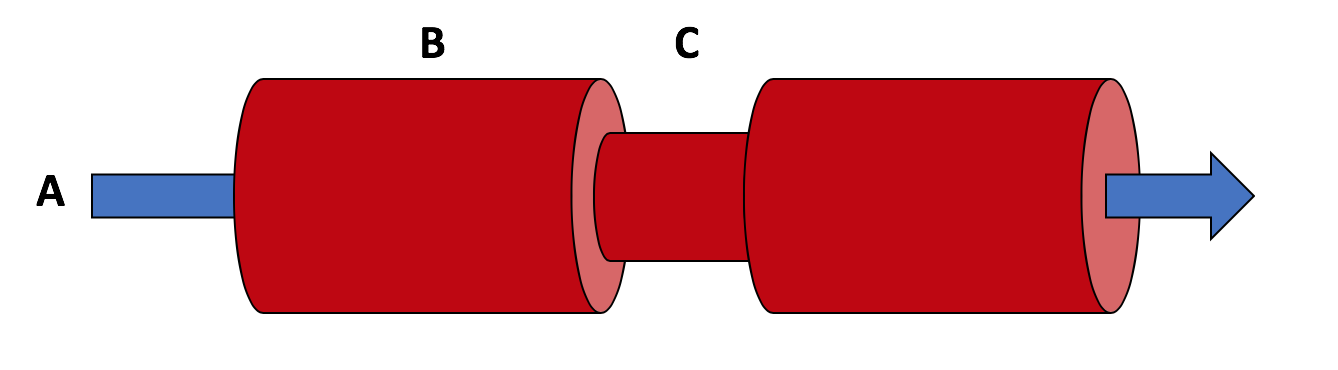
\includegraphics[scale=0.3]{DavidPineiro/stenosis_vein.png}
\centering
\caption{Example artery stenosis we simulate on this report. (A) corresponds to an arrow symbolizing the flow of blood through a vein, (B) demonstrates the normal size of the artery, and (C) highlights the stenosis, a part of the artery which is constricted.}
\label{fig:stenosis_example}
\end{figure}

\subsection{Lattice-Boltzmann Method}
The Lattice-Boltzmann method (LBM) was a natural deduction from Ludwig Boltzmann’s kinetic theory of gases. The method fundamentally understands liquids and gases as a collection of particles undergoing random motions. These particles exchange momentum through particle streaming and inelastic collisions. LBM reduces Boltzmann’s gas dynamics by decreasing the number of particles and confining them to a lattice. In the case of a two dimensional model, particles are restricted to stream in nine directions, including the one for staying in place. This report further delves into the LBM on the section regarding the numerical methods utilized. 


Numerically solving the Boltzmann equation has advantages over numerically solving the Navier-Stokes equations. LBM allows the computation to neglect the nonlinear term, further reducing the amount of computation needed. The method further allows parallelization, which we take advantage of to speed up computation in GPUs and CPUs. LBM remains an upcoming simulation technique for modelling complex fluid systems. LBM has especially gained traction from computational physicists who are able to simulate dynamic problems which would otherwise take larger amounts of time.  